%%%%%%%%%%%%%%%%%%%%%%%%%%%%%%%%%%%%%%%%%%%%%%%%%%%%%%%%%%%%%%%%%%%%%%
% How to use writeLaTeX: 
%
% You edit the source code here on the left, and the preview on the
% right shows you the result within a few seconds.
%
% Bookmark this page and share the URL with your co-authors. They can
% edit at the same time!
%
% You can upload figures, bibliographies, custom classes and
% styles using the files menu.
%
%%%%%%%%%%%%%%%%%%%%%%%%%%%%%%%%%%%%%%%%%%%%%%%%%%%%%%%%%%%%%%%%%%%%%%

\documentclass[12pt]{article}

\usepackage{sbc-template}

\usepackage{graphicx,url}

%\usepackage[brazil]{babel}   
\usepackage[utf8]{inputenc} 

\usepackage{float}
\usepackage{hyperref}
     
\sloppy

\title{Acionamento de Botão Utilizando Multiprocessamento (Thread) + Telegram}

\author{Fabricio Araújo Dias}

\address{Instituto Federal de Educação, Ciência e Tecnologia do Ceará
  (IFCE)\\
  Avenida Vice-Presidente José Alencar, S/N -- 61.939-140 -- Maracanaú -- CE -- Brasil
  \email{fabricio.araujo61@aluno.ifce.edu.br}
}

\begin{document} 

\maketitle

\begin{abstract}
  This report describes the step-by-step practical activity for the Microcontrollers course, which consists of implementing a traffic light for cars and pedestrians using two LEDs and a button and sending a message to Telegram using a button. Both being done at the same time. It is necessary to create tasks and take advantage of multiprocessing, as well as connecting the ESP32 to the internet.
\end{abstract}
     
\begin{resumo} 
  Esse relatório descreve o passo a passo da atividade prática da disciplina de Microcontroladores que consiste em implementar um semáforo para carros e pedestres utilizando dois LEDS e um botão e enviar uma mensagem para o Telegram utilizando um botão. Os dois sendo feitos ao mesmo tempo. Sendo necessário criar tasks e aproveitar o multiprocessamento, assimo como conectar o ESP32 à internet.
\end{resumo}


\section{Introdução}\label{sec:introdução}
A terceira atividade prática consiste em trabalhar com o multiprocessamento do ESP32, visto que ele possui dois cores. A atividade passada será reaproveitada para que funcione em um core, e o outro core irá enviar uma mensagem para uma conta no Telegram por meio de um bot.

\section{Desenvolvimento do Código}\label{sec:desenvolvimento-do-código}

Foram definidos novamente as constantes dos pinos para os LEDs e o botão que são os mesmos da atividade passada. O LED do semáforo dos carros utiliza os pinos 21, 22 e 23; o LED do semáforo dos pedestres utilizam os pinos 33, 32 e 26; e o botão utiliza o pino 19. As constantes de tempo de espera continuam 5000 e 2000.

Os pinModes na função setup também permeneceram inalteradas, com exceção do modo do pino do botão que foi alterado de INPUT para INPUT\_PULLDOWN.

\subsection{Multiprocessamento}

E então, foram definidas as funções que serão usadas como tasks. Uma função se chama de semaphore que faz tudo que a atividade passada consistia que é um semáforo para carros e pedestres. A outra função se chama triggering e ela irá mandar uma mensagem para o Telegram toda a vez que o botão for acionado. A lógica dessas duas funções estão dentro de um while infinito, e cada função possui um delay pequeno e arbitrário para não correr riscos de encher a pilha do ESP32.

Feito isso, chegou a parte de transformar essas funções em tasks. Definimos task handles Task1 e Task2 para identificação das tasks. Para a criação das tasks, utilizamos a função xTaskCreatePinnedToCore, que utiliza como o parâmetros: a função para a task, o seu título, o tamanho da pilha, parâmetros (se tiver), a prioriidade, o task handle e o core a ser utilizado. Para o core 0, foi usado a função dos semáforo, tendo prioridade 0 e sem parâmetros. Para o core 1, foi usado a função triggering, com prioridade 1 e se parâmetros também. Para as duas tasks, o tamanho da pilha é de 10000.

\subsection{Conectando a Rede}

O Dev Kit já possui um módulo Wi-Fi para conectar o ESP32 à internet. Não sendo necessário conectar um outro módulo. Para então, realizarmos a conexão com o bot do Telegram e enviar uma mensagem.

\subsubsection{Módulo Wi-Fi}
Então, foi feita a conexão do ESP32 para a rede Wi-Fi. Foi preferível utilizar a rede de dados móvel do meu celular para evitar transtornos com o wi-fi da universidade. Utilizamos a biblioteca Wifi e WifiClientSecure. Definimos constantes para guardar o SSID e a senha da rede. No setup, escolhemos que o módulo Wifi opere no station mode para que ele possa se conectar a um access point, para então conectamos à rede móvel do meu celular. Conferindo se o Wi-fi foi conectado com sucesso, prosseguimos.

\subsubsection{Configuração no Telegram}

\begin{figure}[H]
    \centering
    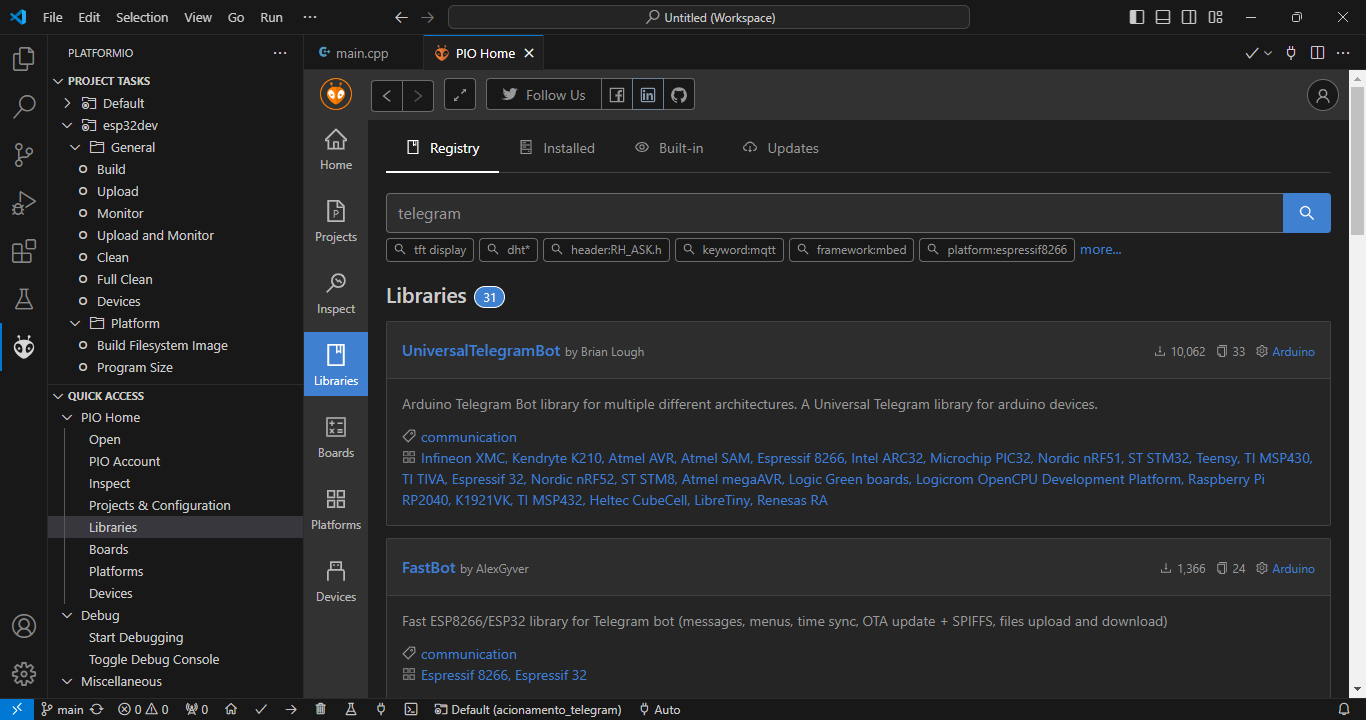
\includegraphics[width=0.5\linewidth]{img/Captura de tela 2024-11-04 215639.png}
    \caption{Tela de busca nas livrarias do PlatformIO.}
    \label{fig:platformIO-libraries}
\end{figure}

Resta preparar o meio para enviar mensagens ao bot do Telegram. Primeiro, instalamos a biblioteca Universal Telegram Bot acessando o menu Libraries na página inicial do PlatformIO. Antes de ir mais afundo, precisamos ir para o aplicativo do Telegram, já possuindo uma conta, e vamos utilizar dois bots: BotFather e IDBot.

\begin{figure}[H]
    \centering
    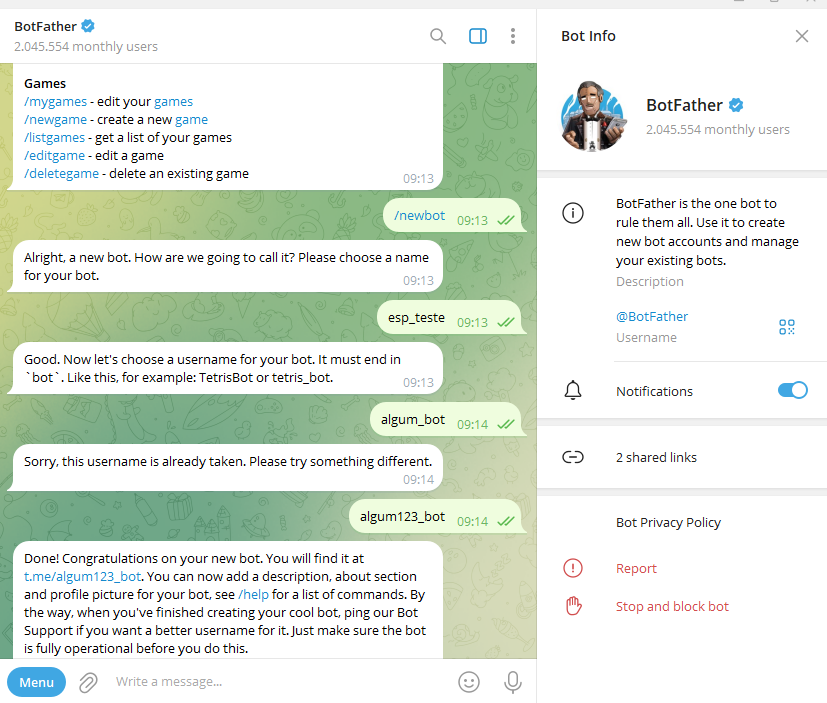
\includegraphics[width=0.5\linewidth]{img/Captura de tela 2024-11-04 215918.png}
    \caption{Chat no Telegram com BotFather.}
    \label{fig:botfather}
\end{figure}

O BotFather é um bot que irá criar um bot para nós de maneira simples. Chamando o bot de apenas "esp\_teste" e um username de "algum123\_bot", ele nos provê um token de acesso à API que será utilizado no código.

O outro bot é o IDBot, que com poucos comandos, nos informa qual o nosso ID no Telegram. É importante para que possamos enviar uma mensagem para nós mesmos.

\subsubsection{Instanciando o Bot}

Voltamos ao código e definimos o token do bot e o nosso ID como constantes. Como variáveis globais, instaciamos um client da classe WifiClientSecure e um bot da classe UniversalTelegramBot - passando como parâmetros o token do bot e o client. Feito isso, o bot está "visível" ao código. Na função triggering, conferimos se o estado do botão é HIGH, e se sim, enviamos uma mensagem para o bot. Para isso, utilizamos o método sendMessage, que recebe como parâmetros: o ID do Telegram, a mensagem e o parse (opcional). Preenchendo com ID do nosso Telegram, uma mensagem qualquer e um vazio, o ESP32 envia uma mensagem para o nosso Telegram.

É possível conferir o código nesse \href{https://github.com/fabricio-araujo94/microcontroladores/tree/main/acionamento_telegram}{repositório do Github}.

\section{Configuração no ESP32}\label{sec:configuração-no-esp32}

Como a atividade prática reutiliza a atividade passada, não houve alterações na configuração do ESP32, com exceção do botão que não é mais ligado a um resistor que liga ao GND. Agora, ele é ligado ao pino 19 e ao pino 3x3 visto que o modo do pino 19 é INPUT\_PULLDOWN.



\section{Considerações Finais}\label{sec:considerações-finais}\hfill

\begin{figure}[H]
    \centering
    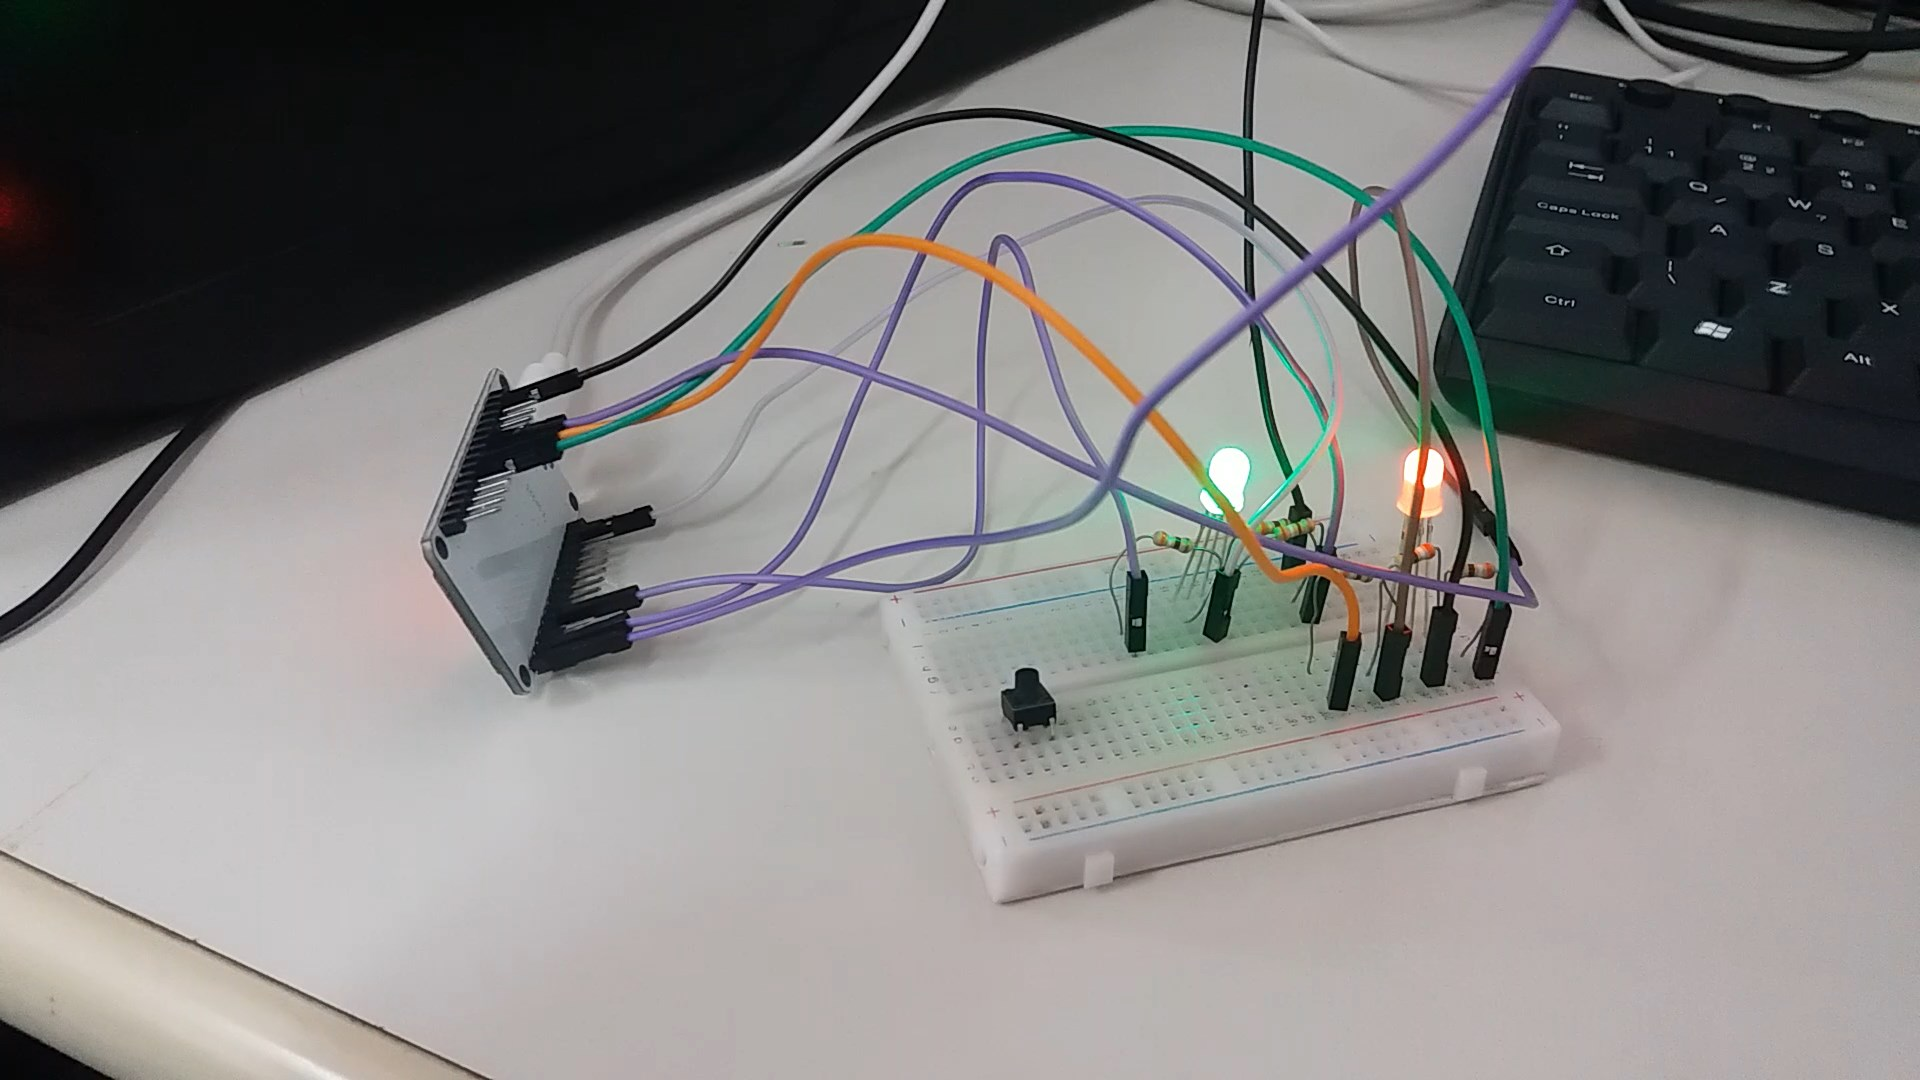
\includegraphics[width=0.5\linewidth]{img/20241030_094251.mp4_snapshot_00.01.049.jpg}
    \caption{Configuração final na protoboard.}
    \label{fig:protoboard}
\end{figure}

Assim, o ESP32 está utilizando um core para manter o semáforo e o outro core para mandar uma mensagem para o Telegram. Isso ao mesmo tempo. Com os dois utilizando o mesmo botão. É possível conferir a execução em vídeo \href{https://youtu.be/ta-vDilDjZk}{aqui}.

\end{document}
